\begin{center}
\underline{\Large{T.P.N°5: Uniones Abulonadas}}
\end{center}

\begin{enumerate}
\item Dimensionar la unión de tipo aplastamiento con bulones de alta resistencia tipo A325, de un
perfil UPN 160 con una cartela de 3/8" de espesor que está sometida a un esfuerzo de
tracción de 450kN. Verificar el bloque de corte. El acero utilizado para los perfiles y la
cartela es F-24.
\begin{figure}[H]
\begin{center}
     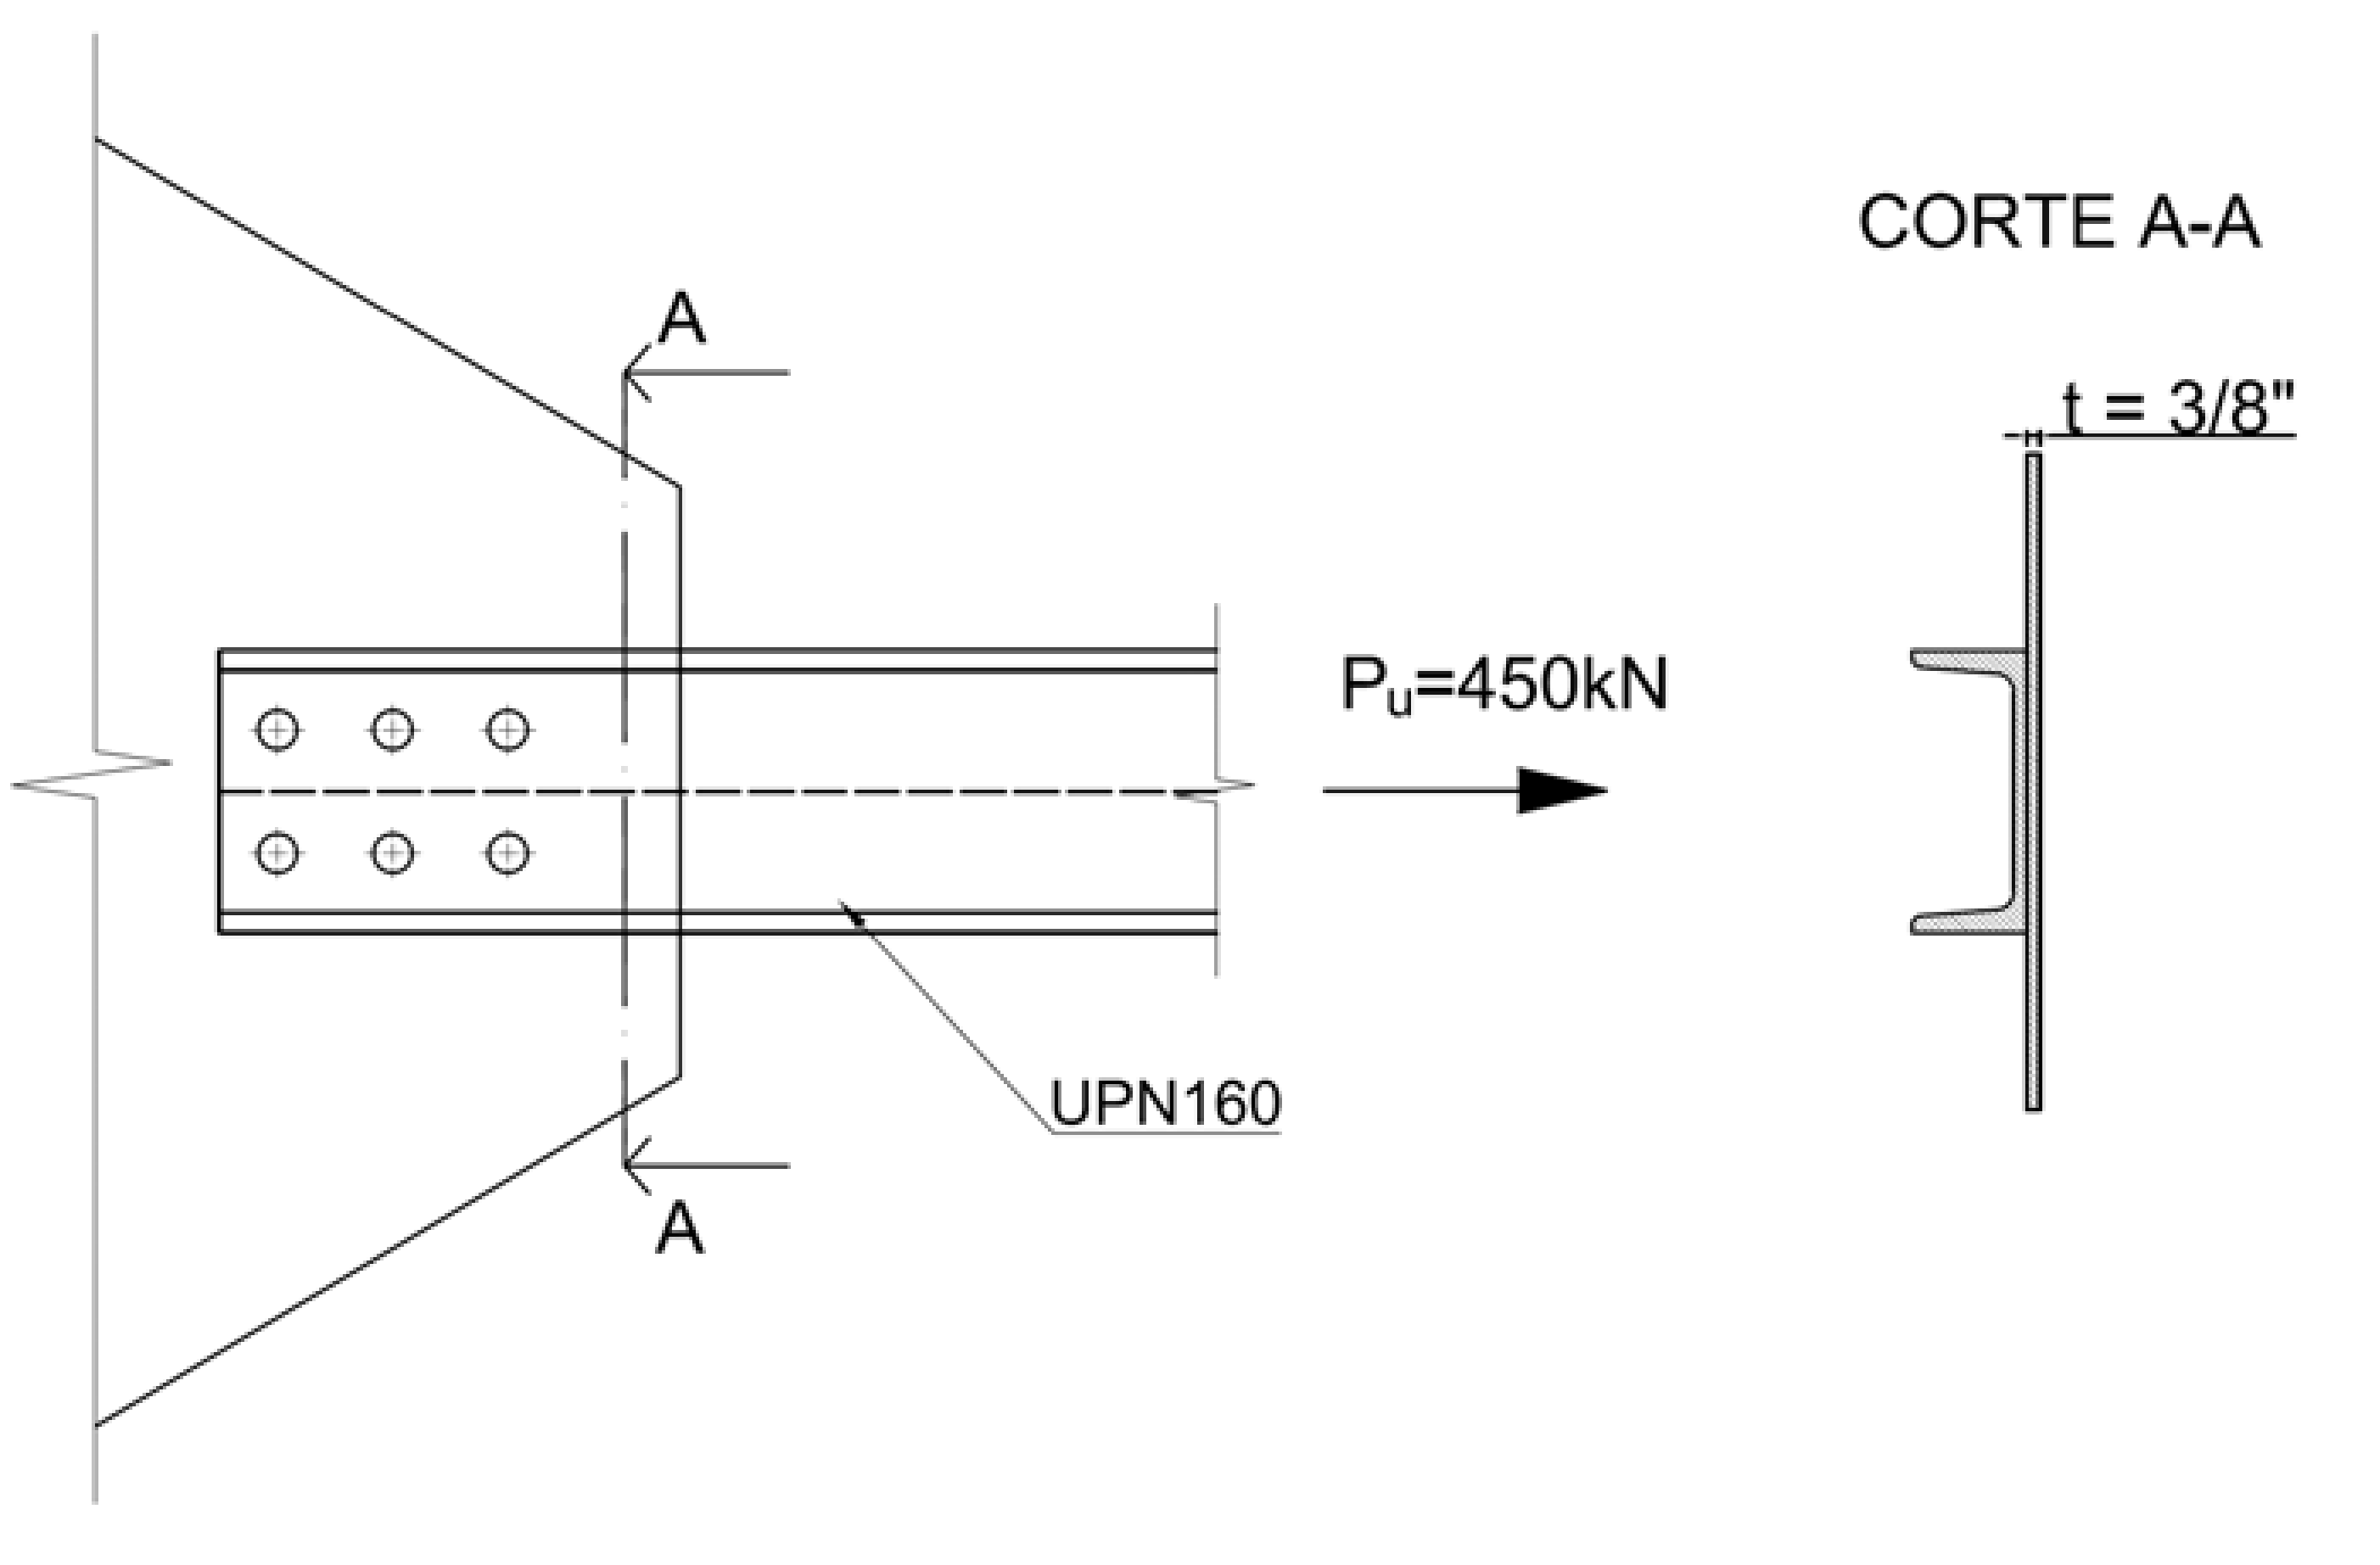
\includegraphics[scale = 1]{chapters/chapter_1/images/figura1.png}
\end{center}
\caption{Unión entre un perfil UPN 160 y una cartela de 3/8"}
\end{figure}
\item Dimensionar la unión de tipo aplastamiento con bulones de alta resistencia de grado 5, entre
una viga principal formada por un IPN240 y una viga secundaria formada por IPN200, que
transmite un esfuerzo de corte de 100kN indicadas en el dibujo. La pieza de unión es un
perfil ángulo de 3" x 3" x 1/4". El material de los perfiles es F-24. Verificar el bloque de
corte.
\begin{figure}[H]
\begin{center}
     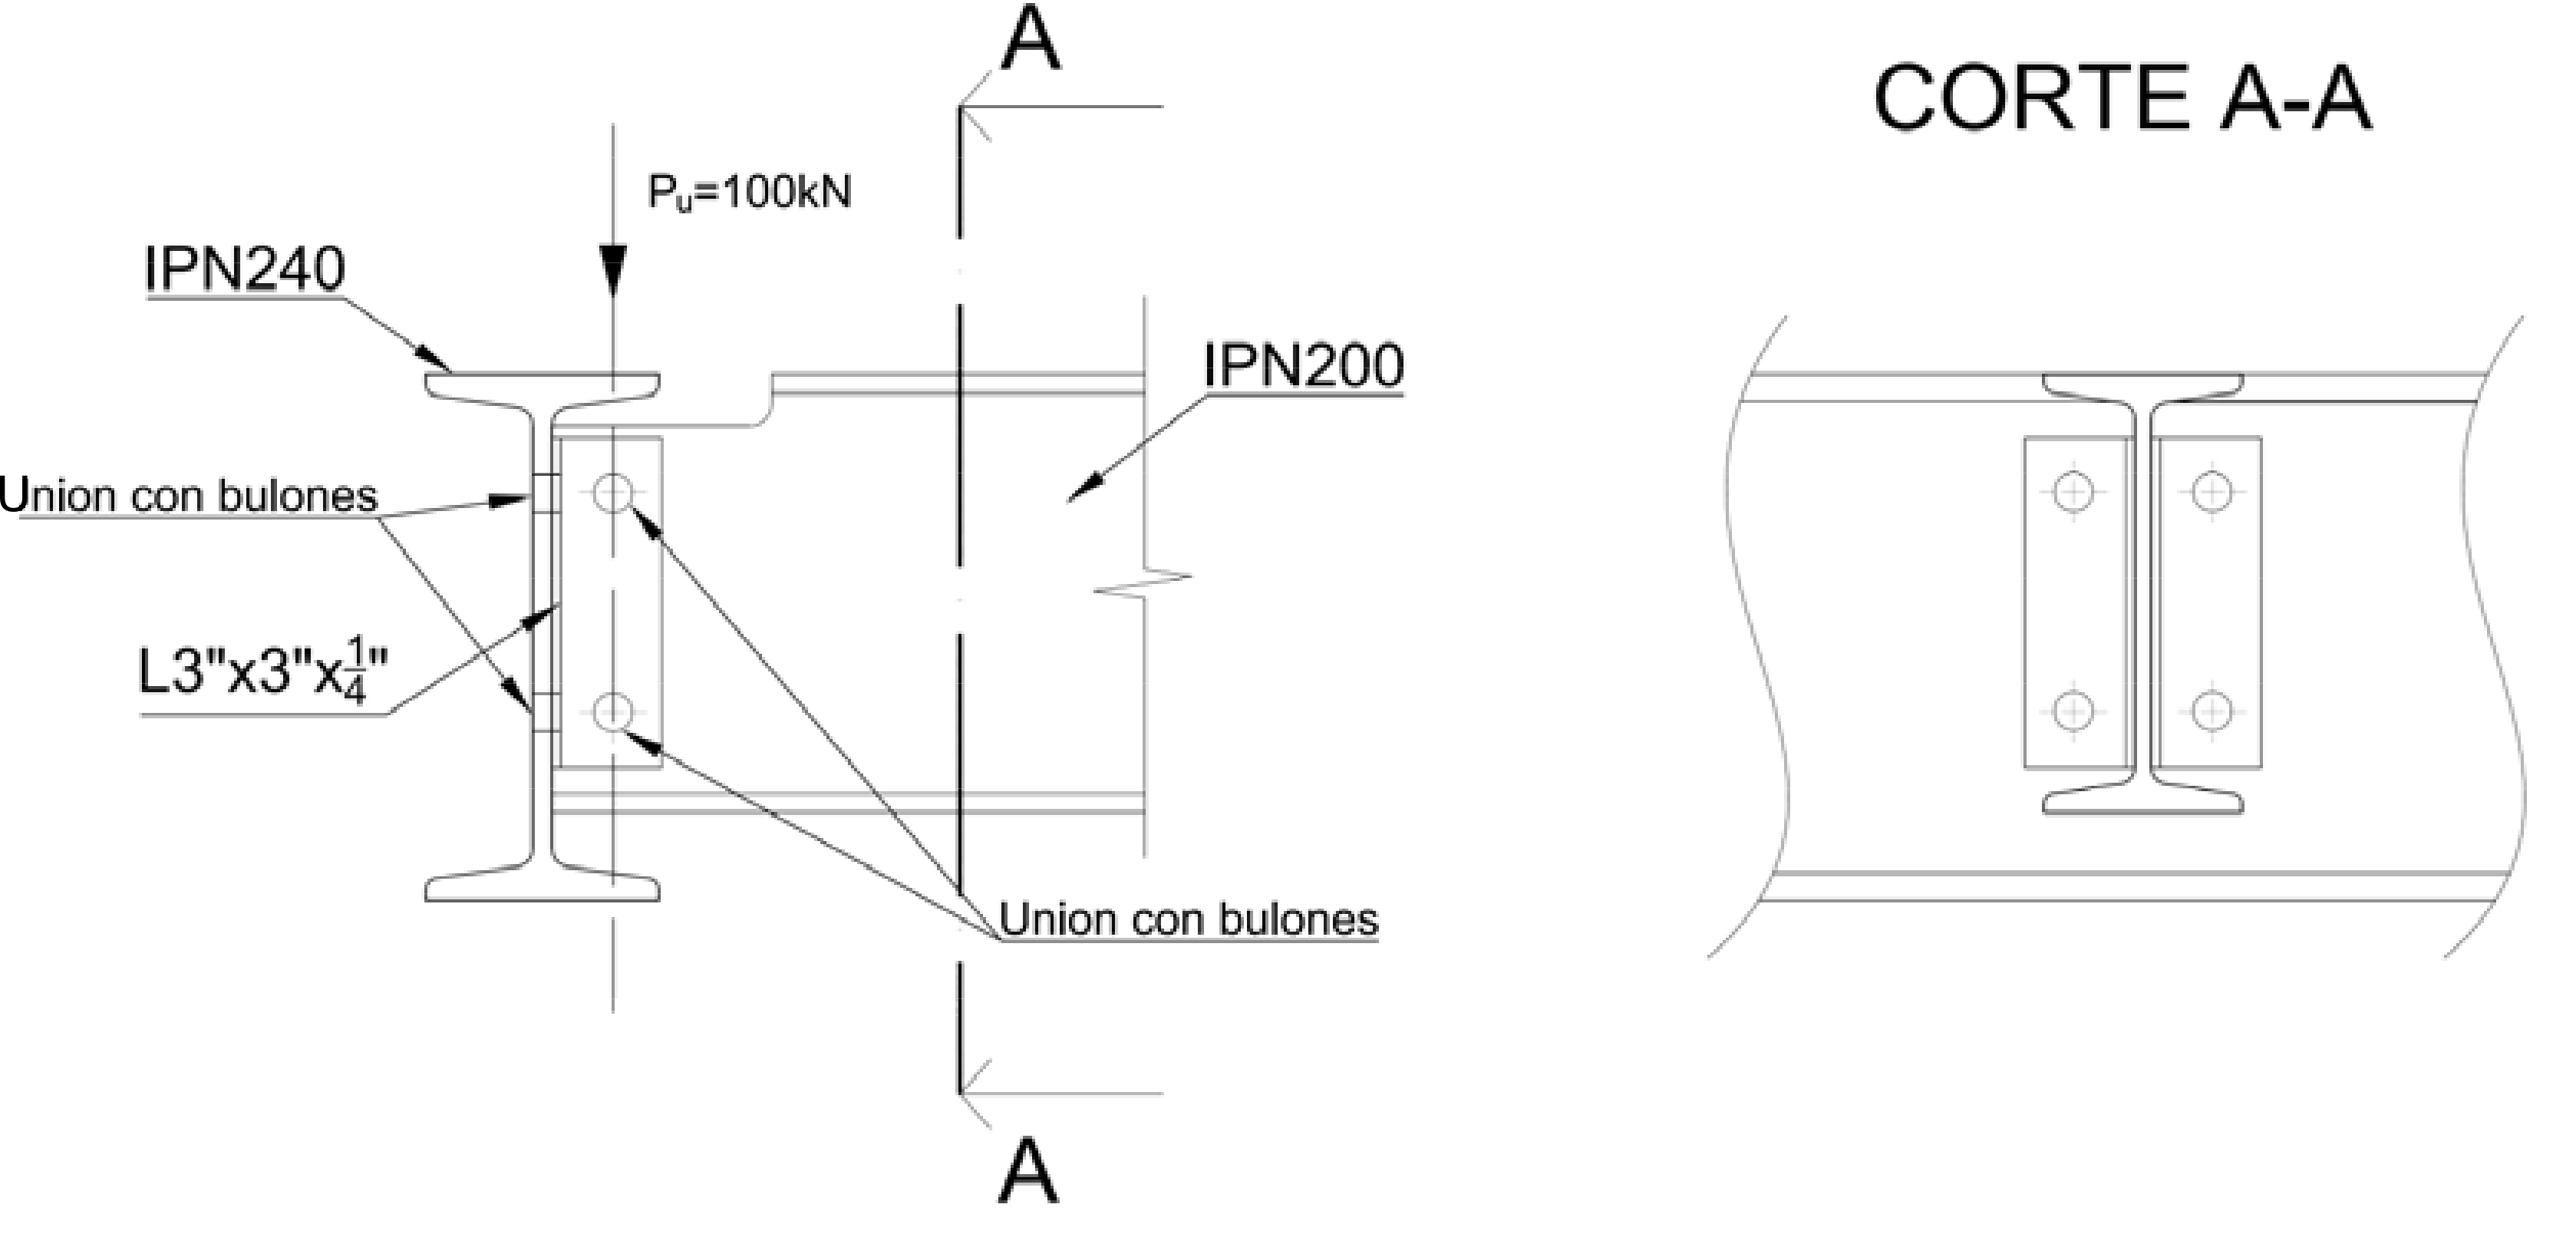
\includegraphics[scale = 1]{chapters/chapter_1/images/figura2.png}
\end{center}
\caption{Unión entre una viga principal IPN240 y una viga secundaria IPN200}
\end{figure}
\end{enumerate}

\newpage

\begin{center}
\underline{\Large{Solución}}
\end{center}

\begin{enumerate}
\item Unión tipo aplastamiento entre un perfil UPN 160 y una cartela de 3/8"
\begin{itemize}
\item \underline{Datos}
\begin{align*}
& \text{Acero F-24}\\
& F_u = 370MPa\\
& F_y = 235MPa
\end{align*}
\begin{align*}
& \text{UPN160}\\
& t_1 = 0.75 cm\\
& \text{Cartela 3/8}\\
& t_2 = 0.952 cm
\end{align*}
\begin{align*}
& \text{Bulón A325}\\
& F_u = 825MPa\\
& F_y = 650MPa
\end{align*}

\begin{figure}[H]
\begin{center}
     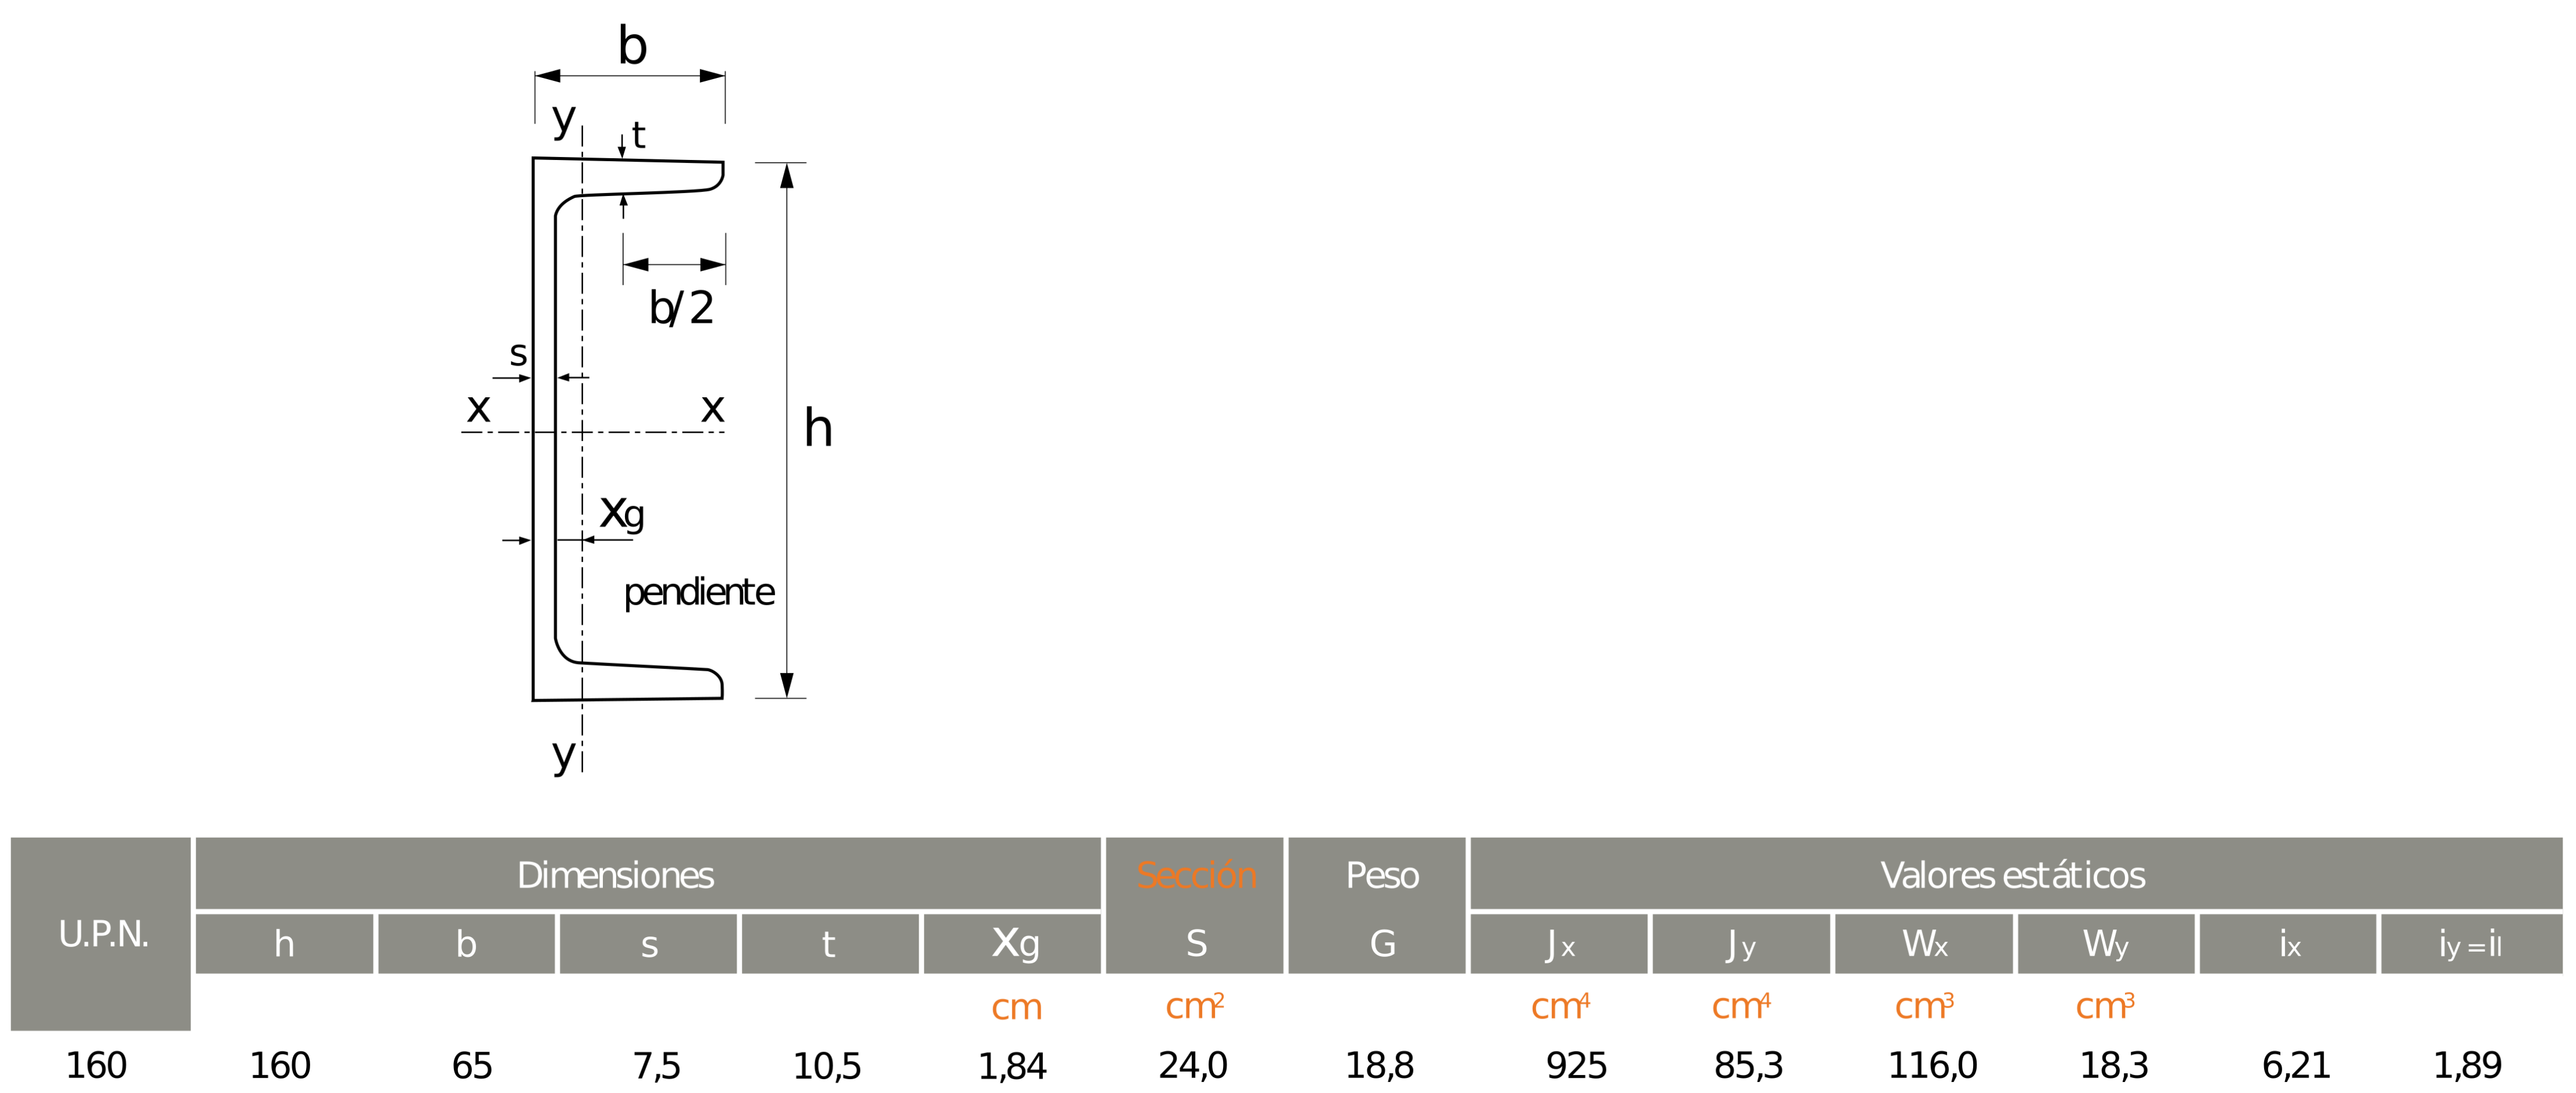
\includegraphics[scale = 0.8]{chapters/chapter_1/images/perfil_UPN160.png}
\end{center}
\caption{Perfil UPN160}
\end{figure}

\begin{figure}[H]
\begin{center}
     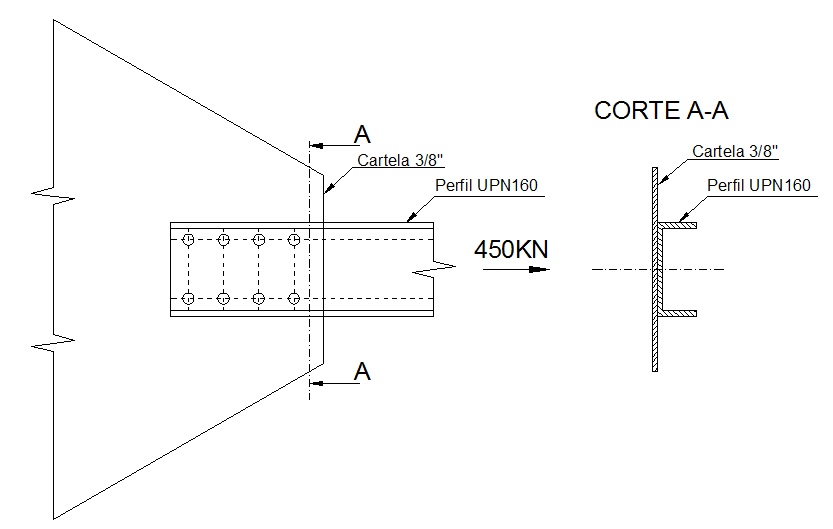
\includegraphics[scale = 0.7]{chapters/chapter_1/images/ejercicio_1.png}
\end{center}
\caption{Unión entre un perfil UPN 160 y una cartela de 3/8"}
\end{figure}


\item \underline{Predimensionado del bulón}
\begin{align*}
& d = \sqrt{5 \cdot t_{min}} - 0.2 = \sqrt{5 \cdot 0.75 cm} - 0.2 = 1.73cm\\
\end{align*}
Adopto bulón 3/4" $\Rightarrow A_b = 2.83 cm^2$ y $\framebox{$d = 1.90 cm$}$ con la rosca fuera del plano de corte.

\item \underline{Resistencia de diseño al corte}
\begin{align*}
& R_d = \phi \cdot F_n \cdot A_b \cdot (10^{-1})\\
& F_n = F_v = 415MPa \quad \text{de tabla J.3.2}\\
& R_d = 0.75 \cdot 415 MPa \cdot 2.83 cm^2 \cdot (10^{-1}) = \framebox{$88.08 KN$}\\
& \text{La cantidad necesaria de bulones es:}\\
& n = \frac{T_u}{R_d} = \frac{450KN}{88.08 KN} = 5.10
\end{align*}
Adopto 8 bulones de 3/4" tipo A325.
\newpage
\item \underline{Distancias y separaciones}
	\begin{itemize}
	\item Distancias mínimas al borde:\\
	Según la tabla J.3.4 para bulones de 3/4 y bordes laminados $d_{borde} = 26 mm$
	\item Separación mínima entre bulones:\\
	$s_{min} = 3 \cdot d = 3 \cdot 1.90cm = 5.70cm$
	\item Separación máxima entre bulones:\\
	Para barras no pintadas de acero resistente a la corrosión atmosférica se debe cumplir:
	\begin{align*}
	& s_{max} \leq 14 \cdot t_{min}\\
	& s_{max} \leq 14 \cdot 0.75cm = 10.5cm\\
	& s_{max} \leq 180mm
	\end{align*}
	\end{itemize}
\item \underline{Verificación al aplastamiento}\\
La resistencia de diseño al aplastamiento de la chapa en los agujeros será:
\begin{align*}
& R_d = \phi \cdot R_n \Rightarrow \text{ con } \phi = 0.75\\
& R_{n1} = 1.2 \cdot L_c \cdot t \cdot F_u \cdot (10^{-1})\\
& R_{n1} = 1.2 \cdot [2 \cdot (3cm - \frac{1.90cm}{2})+ 6 \cdot (6cm - 1.90cm)]\cdot 0.75cm \cdot 370MPa \cdot (10^{-1})\\
& R_{n1} = \framebox{$955.71 KN$}\\
& R_{n2} = 2.4 \cdot d \cdot t \cdot F_u \cdot (10^{-1})\\
& R_{n2} = 2.4 \cdot 1.90cm \cdot 0.75cm \cdot 370MPa \cdot (10^{-1})\\
& R_{n2} = \framebox{$126.54 KN$} \text{ por bulón}\\
& R_{n1} \leq \text{n° de bulones} \cdot R_{n2}\\
& 955.71 KN \leq 8 \cdot 126.54 KN\\
& 955.71 KN \leq 1012.32 KN \quad \surd \quad \text{Verifica}\\
& \Rightarrow R_d = \phi \cdot R_n = 0.75 \cdot 955.71 KN = \framebox{$716.78 KN$}\\
& R_d > T_u\\
& 716.78 KN > 450 KN \quad \surd \quad \text{Verifica}
\end{align*}

\item \underline{Verificación del bloque de corte}

\begin{align*}
& A_{gv} = 2 \cdot 0.75cm \cdot (6cm + 6cm + 6cm + 3cm) = \framebox{$31.50 cm^2$}\\
& A_{nv} = 2 \cdot 0.75cm \cdot [3 \cdot (6cm - 1.90cm) + (3cm - \frac{1.90cm}{2})] = \framebox{$21.53 cm^2$}\\
& A_{gt} = 0.75cm \cdot 10cm = \framebox{$7.5 cm^2$}\\
& A_{nt} = 0.75cm \cdot (10cm - 1.90cm) = \framebox{$6.07 cm^2$}
\end{align*}
Se debe cumplir la condición:
\begin{align*}
& F_u \cdot A_{nt} \cdot (10^{-1}) < 0.6 \cdot F_u \cdot A_{nv} \cdot (10^{-1})\\
& 370MPa \cdot 6.07 cm^2 \cdot (10^{-1}) < 0.6 \cdot 370MPa \cdot 21.53 cm^2 \cdot (10^{-1})\\
& 224.59KN < 477.96KN \quad \surd \quad \text{Verifica}\\
\end{align*}
Entonces la resistencia del bloque de corte viene dada por:
\begin{align*}
& \phi \cdot R_n = \phi \cdot [0.6 \cdot F_u \cdot A_{nv} + F_y \cdot A_{gt}]\cdot (10^{-1})\\
& \phi \cdot R_n = 0.75 \cdot [0.6 \cdot 370MPa \cdot 21.53 cm^2 + 235MPa \cdot 7.5 cm^2]\cdot (10^{-1})\\
& \phi \cdot R_n = \framebox{$490.66 KN$} \quad \surd \quad \text{Verifica}
\end{align*}

\item \underline{Disposición final de la unión}

\begin{figure}[H]
\begin{center}
     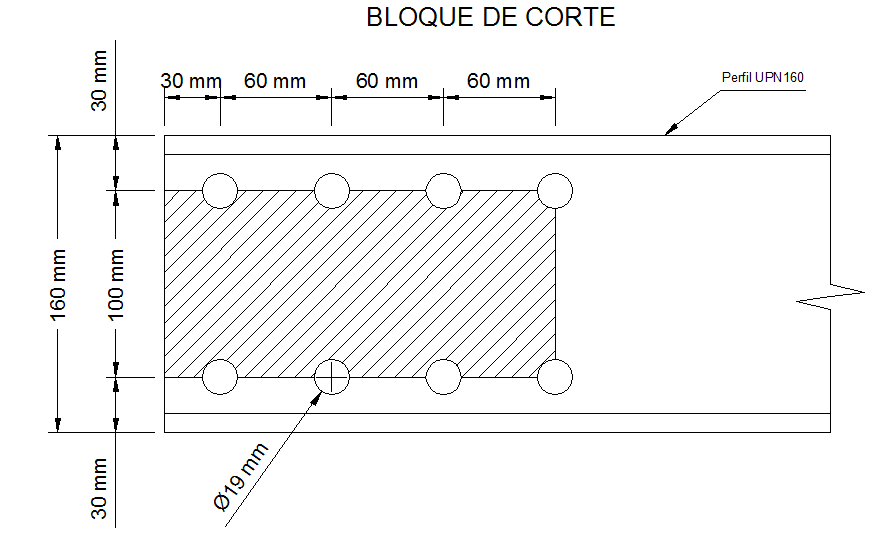
\includegraphics[scale = 0.6]{chapters/chapter_1/images/Bloque_de_Corte_1.png}
\end{center}
\caption{Bloque de Corte}
\end{figure}
\end{itemize}
\newpage
\item Unión tipo aplastamiento entre una viga principal IPN240 y una viga secundaria IPN200
\begin{itemize}
\item \underline{Datos}
\begin{align*}
& \text{Acero F-24}\\
& F_u = 370MPa\\
& F_y = 235MPa
\end{align*}
\begin{align*}
& \text{IPN200}\\
& s_1 = 0.75 cm\\
& \text{IPN240}\\
& s_2 = 0.87 cm\\
& \text{Perfil L 3x1/4}\\
& e_3 = 0.64 cm
\end{align*}
\begin{align*}
& \text{Bulón Grado 5}\\
& F_u = 840MPa\\
& F_y = 670MPa
\end{align*}

\begin{figure}[H]
\begin{center}
     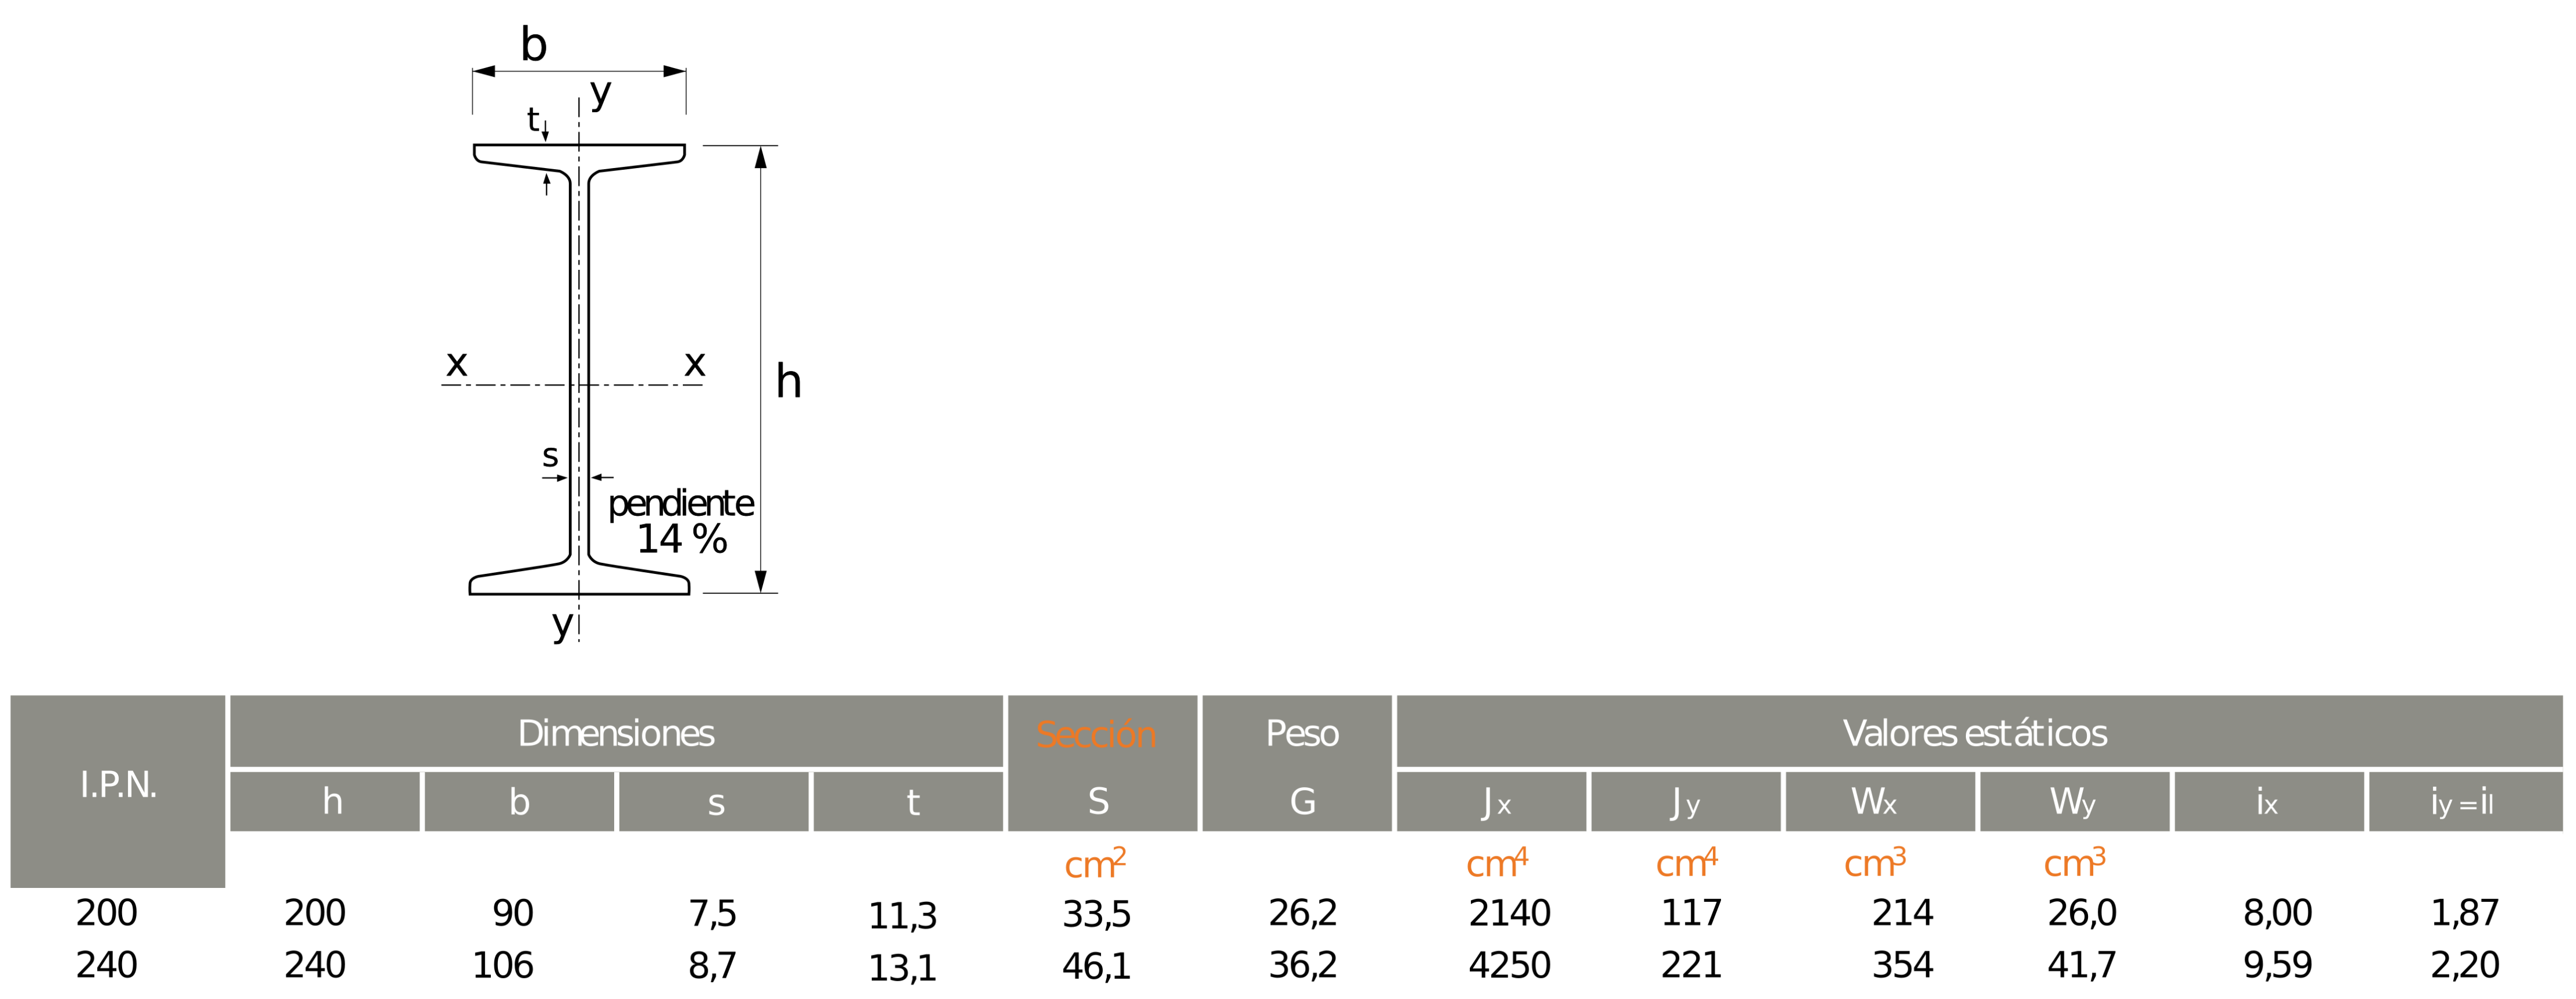
\includegraphics[scale = 0.8]{chapters/chapter_1/images/perfil_IPN.png}
\end{center}
\caption{Perfiles IPN200 e IPN240}
\end{figure}

\begin{figure}[H]
\begin{center}
     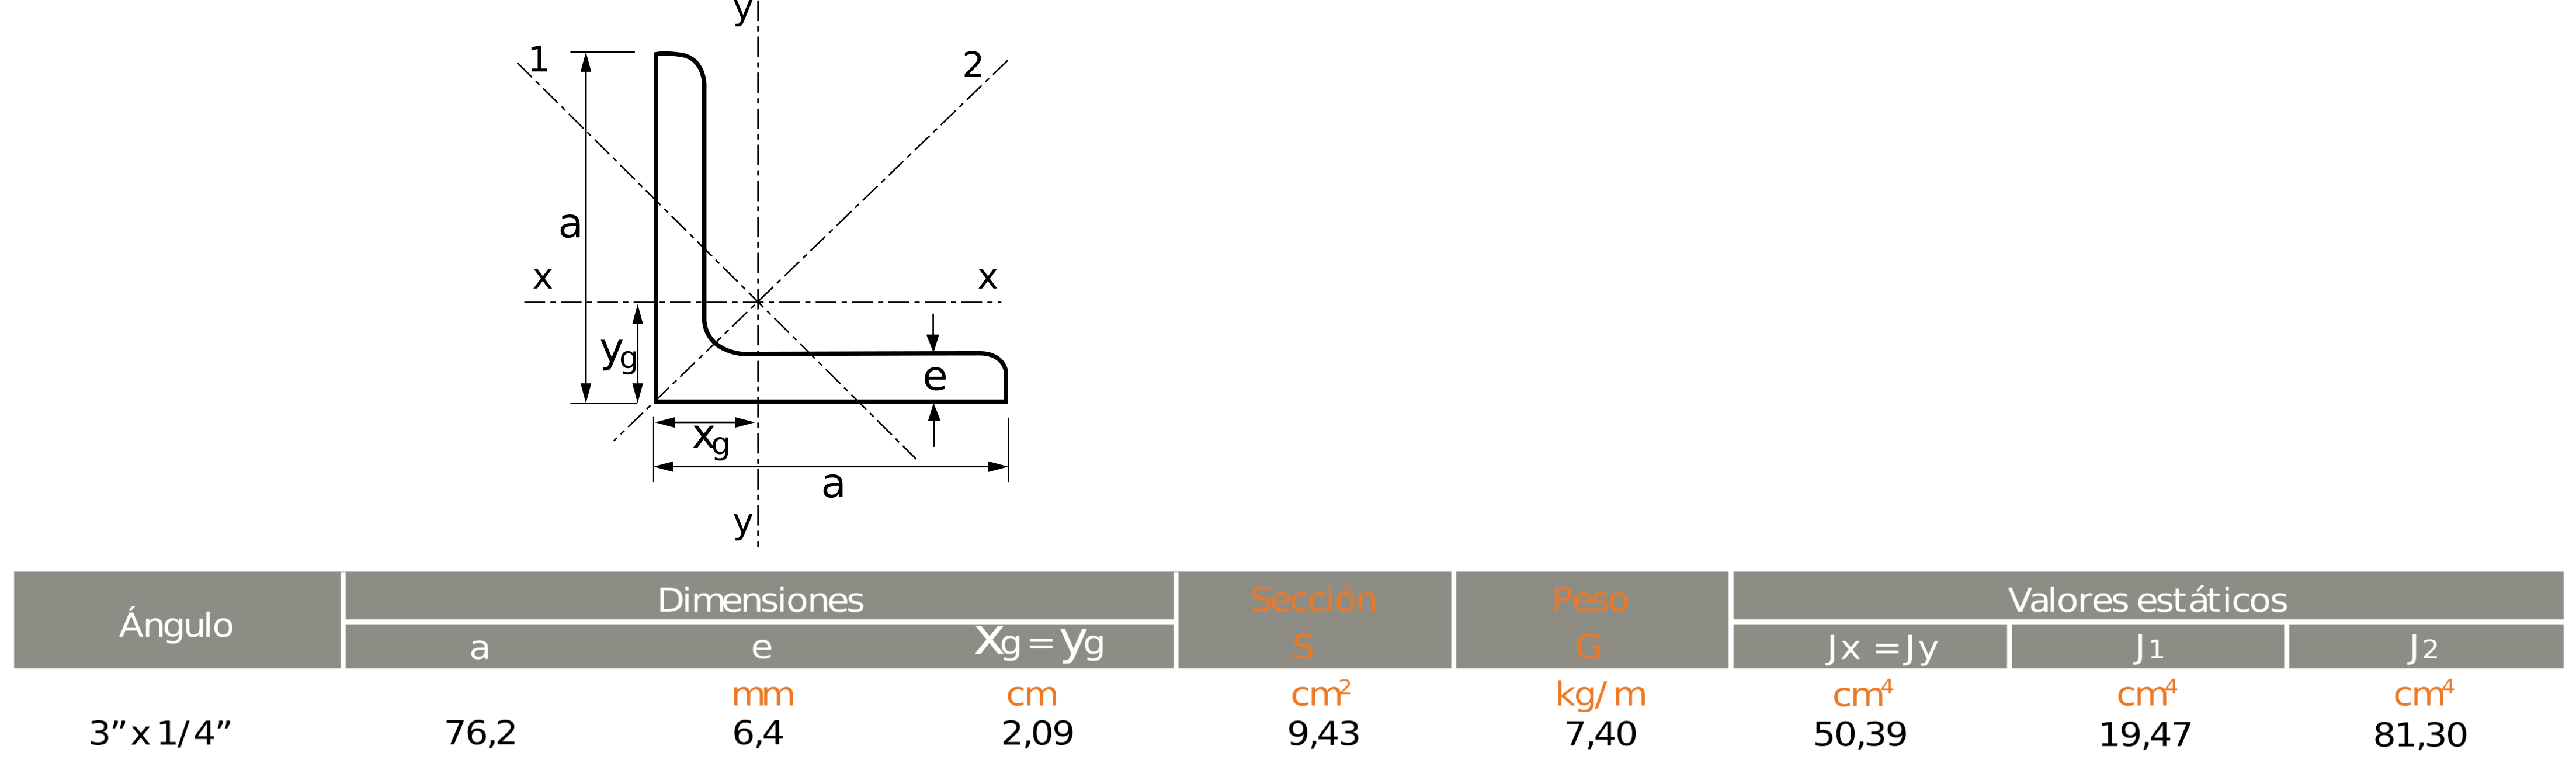
\includegraphics[scale = 0.8]{chapters/chapter_1/images/perfil_angulo.png}
\end{center}
\caption{Perfil L 3"x1/4"}
\end{figure}

\begin{figure}[H]
\begin{center}
     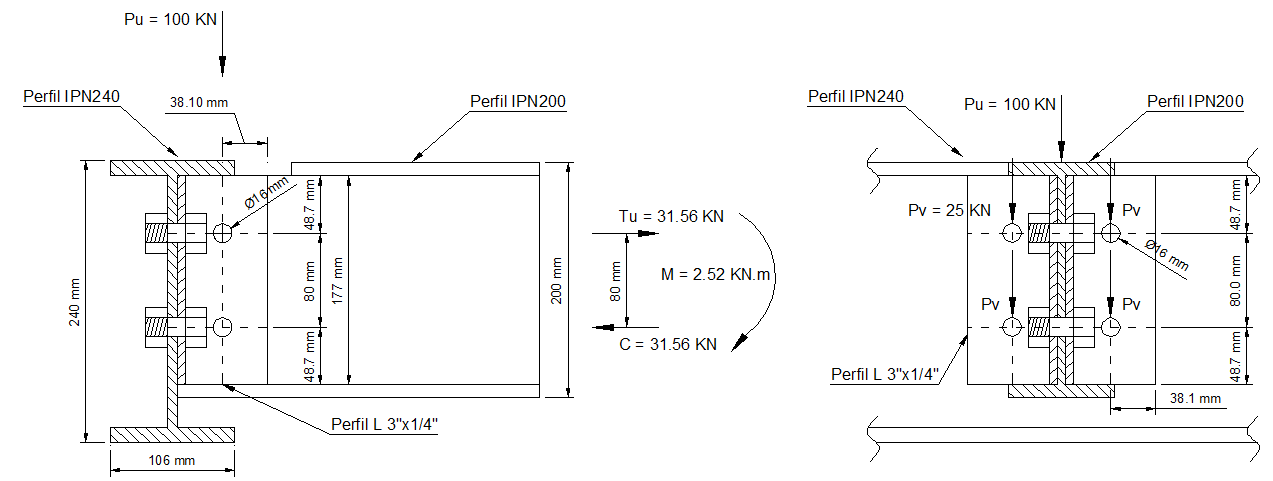
\includegraphics[scale = 0.5]{chapters/chapter_1/images/ejercicio_2.png}
\end{center}
\caption{Unión entre una viga principal IPN240 y una viga secundaria IPN200}
\end{figure}

\begin{center}
\underline{UNION CON LA VIGA SECUNDARIA}\\
\underline{VERIFICACIÓN AL CORTE}
\end{center}

\item \underline{Predimensionado del bulón}
\begin{align*}
& d = \sqrt{5 \cdot t_{min}} - 0.2 = \sqrt{5 \cdot 0.64 cm} - 0.2 = 1.58cm\\
\end{align*}
Adopto bulón 5/8" $\Rightarrow A_b = 1.98 cm^2$ y $\framebox{$d = 1.587 cm$}$ con la rosca fuera del plano de corte.

\item \underline{Resistencia de diseño al corte}
\begin{align*}
& R_d = \phi \cdot F_n \cdot A_b \cdot (10^{-1})\\
& F_n = F_v = 415MPa \quad \text{de tabla J.3.2}\\
& R_d = 0.75 \cdot 415 MPa \cdot 1.98 cm^2 \cdot (10^{-1}) = \framebox{$61.62 KN$}\\
& \text{La cantidad necesaria de bulones es:}\\
& n = \frac{P_u}{R_d} = \frac{100KN}{61.62KN} = 1.62
\end{align*}
Adopto 2 bulones de 5/8" tipo SAE Grado 5.

\item \underline{Distancias y separaciones}
	\begin{itemize}
	\item Distancias mínimas al borde:\\
	Según la tabla J.3.4 para bulones de 5/8 y bordes laminados $d_{borde} = 22 mm$
	\item Separación mínima entre bulones:\\
	$s_{min} = 3 \cdot d = 3 \cdot 1.587cm = 4.76cm$
	\item Separación máxima entre bulones:\\
	Para barras no pintadas de acero resistente a la corrosión atmosférica se debe cumplir:
	\begin{align*}
	& s_{max} \leq 14 \cdot t_{min}\\
	& s_{max} \leq 14 \cdot 0.64cm = 8.96cm\\
	& s_{max} \leq 180mm
	\end{align*}
	\end{itemize}

\item \underline{Verificación al aplastamiento}\\
La resistencia de diseño al aplastamiento de la chapa en los agujeros será:
\begin{align*}
& R_d = \phi \cdot R_n \Rightarrow \text{ con } \phi = 0.75\\
& R_{n1} = 1.2 \cdot L_c \cdot t \cdot F_u \cdot (10^{-1})\\
& R_{n1} = 1.2 \cdot [(4.87cm - \frac{1.587cm}{2})+ (8cm - 1.587cm)]\cdot 0.64cm \cdot 370MPa \cdot (10^{-1})\\
& R_{n1} = \frac{298.07KN}{2 \cdot \text{perfiles}} = \framebox{$149.03 KN$}\\
& R_{n2} = 2.4 \cdot d \cdot t \cdot F_u \cdot (10^{-1})\\
& R_{n2} = 2.4 \cdot 1.587cm \cdot 0.64cm \cdot 370MPa \cdot (10^{-1})\\
& R_{n2} = \framebox{$90.19 KN$} \text{ por bulón}\\
& R_{n1} \leq \text{n° de bulones} \cdot R_{n2}\\
& 149.03 KN \leq 2 \cdot 90.19 KN\\
& 149.03 KN \leq 180.38 KN \quad \surd \quad \text{Verifica}\\
& \Rightarrow R_d = \phi \cdot R_n = 0.75 \cdot 149.03 KN = \framebox{$111.77 KN$}\\
& R_d > \frac{P_u}{2}\\
& 111.77 KN > 50 KN \quad \surd \quad \text{Verifica}
\end{align*}

\item \underline{Verificación del bloque de corte}

\begin{align*}
& A_{gv} = 0.64cm \cdot (8cm + 4.87cm) = \framebox{$8.24 cm^2$}\\
& A_{nv} = 0.64cm \cdot [(8cm - 1.587cm) + (4.87cm - \frac{1.587cm}{2})] = \framebox{$6.71 cm^2$}\\
& A_{gt} = 0.64cm \cdot 3.81cm = \framebox{$2.43 cm^2$}\\
& A_{nt} = 0.64cm \cdot (3.81cm - \frac{1.587cm}{2}) = \framebox{$1.93 cm^2$}
\end{align*}
Se debe cumplir la condición:
\begin{align*}
& F_u \cdot A_{nt} \cdot (10^{-1}) < 0.6 \cdot F_u \cdot A_{nv} \cdot (10^{-1})\\
& 370MPa \cdot 1.93 cm^2 \cdot (10^{-1}) < 0.6 \cdot 370MPa \cdot 6.71 cm^2 \cdot (10^{-1})\\
& 71.41KN < 148.96KN \quad \surd \quad \text{Verifica}\\
\end{align*}
Entonces la resistencia del bloque de corte viene dada por:
\begin{align*}
& \phi \cdot R_n = \phi \cdot [0.6 \cdot F_u \cdot A_{nv} + F_y \cdot A_{gt}]\cdot (10^{-1})\\
& \phi \cdot R_n = 0.75 \cdot [0.6 \cdot 370MPa \cdot 6.71 cm^2 + 235MPa \cdot 2.43 cm^2]\cdot (10^{-1})\\
& \phi \cdot R_n = \framebox{$154.55 KN$} \quad \surd \quad \text{Verifica}
\end{align*}

\begin{figure}[H]
\begin{center}
     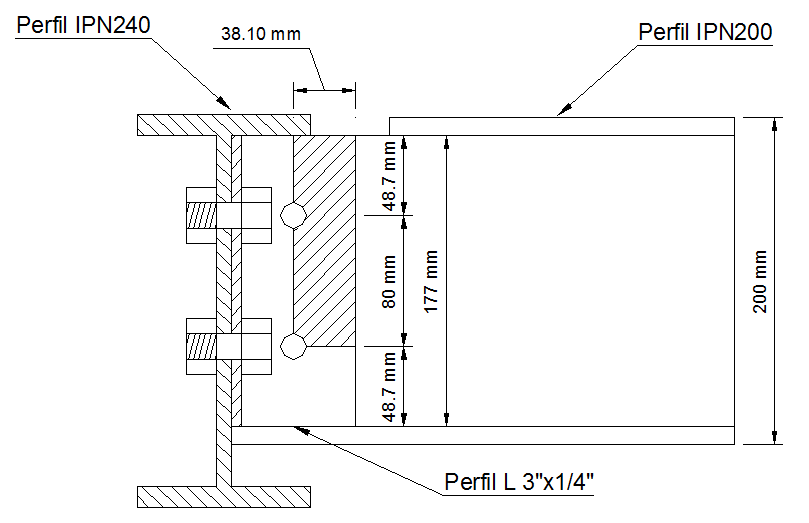
\includegraphics[scale = 0.6]{chapters/chapter_1/images/Bloque_de_Corte_2.png}
\end{center}
\caption{Bloque de Corte}
\end{figure}

\item \underline{Verificación del bloque de corte del alma de la viga secundaria IPN200}

\begin{align*}
& A_{gv} = 0.75cm \cdot (8cm + 4.87cm) = \framebox{$9.65 cm^2$}\\
& A_{nv} = 0.75cm \cdot [(8cm - 1.587cm) + (4.87cm - \frac{1.587cm}{2})] = \framebox{$7.87 cm^2$}\\
& A_{gt} = 0.75cm \cdot 3.81cm = \framebox{$2.86 cm^2$}\\
& A_{nt} = 0.75cm \cdot (3.81cm - \frac{1.587cm}{2}) = \framebox{$2.26 cm^2$}
\end{align*}
Se debe cumplir la condición:
\begin{align*}
& F_u \cdot A_{nt} \cdot (10^{-1}) < 0.6 \cdot F_u \cdot A_{nv} \cdot (10^{-1})\\
& 370MPa \cdot 2.26 cm^2 \cdot (10^{-1}) < 0.6 \cdot 370MPa \cdot 7.87 cm^2 \cdot (10^{-1})\\
& 83.71KN < 174.65KN \quad \surd \quad \text{Verifica}\\
\end{align*}
Entonces la resistencia del bloque de corte viene dada por:
\begin{align*}
& \phi \cdot R_n = \phi \cdot [0.6 \cdot F_u \cdot A_{nv} + F_y \cdot A_{gt}]\cdot (10^{-1})\\
& \phi \cdot R_n = 0.75 \cdot [0.6 \cdot 370MPa \cdot 7.87 cm^2 + 235MPa \cdot 2.86 cm^2]\cdot (10^{-1})\\
& \phi \cdot R_n = \framebox{$181.35 KN$} \quad \surd \quad \text{Verifica}
\end{align*}

\begin{figure}[H]
\begin{center}
     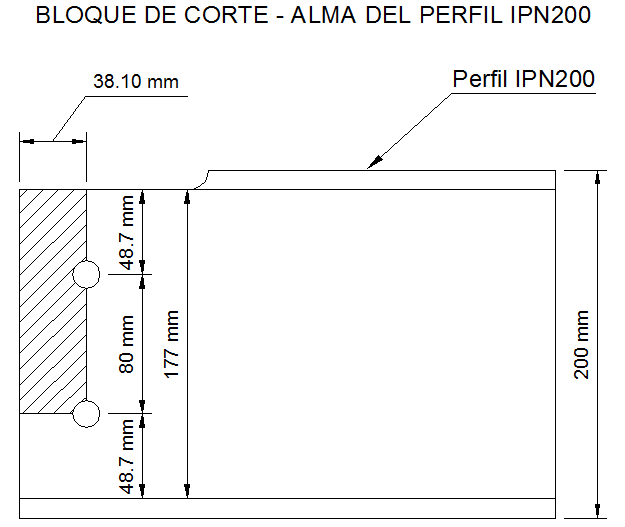
\includegraphics[scale = 0.6]{chapters/chapter_1/images/Bloque_de_Corte_4.png}
\end{center}
\caption{Bloque de Corte}
\end{figure}

\newpage
\begin{center}
\underline{UNION CON LA VIGA PRINCIPAL}\\
\underline{VERIFICACIÓN A TRACCIÓN Y CORTE COMBINADOS}
\end{center}

\item \underline{Predimensionado del bulón}
\begin{align*}
& d = \sqrt{5 \cdot t_{min}} - 0.2 = \sqrt{5 \cdot 0.64 cm} - 0.2 = 1.58cm\\
\end{align*}
Adopto bulón 5/8" $\Rightarrow A_b = 1.98 cm^2$ y $\framebox{$d = 1.587 cm$}$ con la rosca fuera del plano de corte.

\item \underline{Distancias y separaciones}
	\begin{itemize}
	\item Distancias mínimas al borde:\\
	Según la tabla J.3.4 para bulones de 5/8 y bordes laminados $d_{borde} = 22 mm$
	\item Separación mínima entre bulones:\\
	$s_{min} = 3 \cdot d = 3 \cdot 1.587cm = 4.76cm$
	\item Separación máxima entre bulones:\\
	Para barras no pintadas de acero resistente a la corrosión atmosférica se debe cumplir:
	\begin{align*}
	& s_{max} \leq 14 \cdot t_{min}\\
	& s_{max} \leq 14 \cdot 0.64cm = 8.96cm\\
	& s_{max} \leq 180mm
	\end{align*}
	\end{itemize}

\item \underline{Estado de cargas}

\begin{align*}
& M = P_u \cdot (X_g + \frac{s_2}{2}) \\
& M = 100KN \cdot (2.09cm + \frac{0.87cm}{2}) \cdot \frac{1m}{100cm} = \framebox{$2.52KN \cdot m$} \\
& T_u = \frac{M}{z} = \frac{2.52KN \cdot m}{0.08m} = \framebox{$31.56 KN$} \quad \text{Tomado con dos bulones}\\
& P_v = \frac{P_u}{4} = \frac{100KN}{4} = \framebox{$25 KN$} \quad \text{Tomado con cuatro bulones}
\end{align*}
\newpage
\item \underline{Resistencia a Tracción y Corte combinados}

\begin{align*}
& F_v = \frac{P_v}{A_b \cdot 10^{-1}} = \frac{25 KN}{1.98 cm^2 \cdot 10^{-1}} = \framebox{$126.26 MPa$}\\
& F_t = 808 - 2 \cdot F_v = 808 - 2 \cdot 126.26 MPa = \framebox{$555.48 MPa$} \\
& F_t \leq 620 MPa \\
& 555.48 MPa \leq 620 MPa \quad \surd \quad \text{Verifica} \\
& R_d = 0.75 \cdot F_t \cdot A_b \cdot 10^{-1} = 0.75 \cdot 555.48 MPa \cdot 1.98 cm^2 \cdot 10^{-1} = \framebox{$82.48 KN$}\\
& R_d \geq \frac{T_u}{2}\\
& 82.48 KN \geq \frac{31.56 KN}{2}\\
& 82.48 KN \geq 15.78 KN \quad \surd \quad \text{Verifica} \\
\end{align*}

\item \underline{Verificación al aplastamiento}\\
La resistencia de diseño al aplastamiento de la chapa en los agujeros será:
\begin{align*}
& R_d = \phi \cdot R_n \Rightarrow \text{ con } \phi = 0.75\\
& R_{n1} = 1.2 \cdot L_c \cdot t \cdot F_u \cdot (10^{-1})\\
& R_{n1} = 1.2 \cdot (4.87cm - \frac{1.587cm}{2}) \cdot 0.64cm \cdot 370MPa \cdot (10^{-1})\\
& R_{n1} = \framebox{$115.83 KN$}\\
& R_{n2} = 2.4 \cdot d \cdot t \cdot F_u \cdot (10^{-1})\\
& R_{n2} = 2.4 \cdot 1.587cm \cdot 0.64cm \cdot 370MPa \cdot (10^{-1})\\
& R_{n2} = \framebox{$90.19 KN$} \text{ por bulón}\\
& R_{n1} \leq \text{n° de bulones} \cdot R_{n2}\\
& 115.83 KN \leq 2 \cdot 90.19 KN\\
& 115.83 KN \leq 180.38 KN \quad \surd \quad \text{Verifica}\\
& \Rightarrow R_d = \phi \cdot R_n = 0.75 \cdot 115.83 KN = \framebox{$86.87 KN$}\\
& R_d > P_v\\
& 86.87 KN > 25 KN \quad \surd \quad \text{Verifica}
\end{align*}
\newpage
\item \underline{Verificación del bloque de corte}

\begin{align*}
& A_{gv} = 0.64cm \cdot (8cm + 4.87cm) = \framebox{$8.24 cm^2$}\\
& A_{nv} = 0.64cm \cdot [(8cm - 1.587cm) + (4.87cm - \frac{1.587cm}{2})] = \framebox{$6.71 cm^2$}\\
& A_{gt} = 0.64cm \cdot 3.81cm = \framebox{$2.43 cm^2$}\\
& A_{nt} = 0.64cm \cdot (3.81cm - \frac{1.587cm}{2}) = \framebox{$1.93 cm^2$}
\end{align*}
Se debe cumplir la condición:
\begin{align*}
& F_u \cdot A_{nt} \cdot (10^{-1}) < 0.6 \cdot F_u \cdot A_{nv} \cdot (10^{-1})\\
& 370MPa \cdot 1.93 cm^2 \cdot (10^{-1}) < 0.6 \cdot 370MPa \cdot 6.71 cm^2 \cdot (10^{-1})\\
& 71.41KN < 148.96KN \quad \surd \quad \text{Verifica}\\
\end{align*}
Entonces la resistencia del bloque de corte viene dada por:
\begin{align*}
& \phi \cdot R_n = \phi \cdot [0.6 \cdot F_u \cdot A_{nv} + F_y \cdot A_{gt}]\cdot (10^{-1})\\
& \phi \cdot R_n = 0.75 \cdot [0.6 \cdot 370MPa \cdot 6.71 cm^2 + 235MPa \cdot 2.43 cm^2]\cdot (10^{-1})\\
& \phi \cdot R_n = \framebox{$154.55 KN$} \quad \surd \quad \text{Verifica}
\end{align*}

\begin{figure}[H]
\begin{center}
     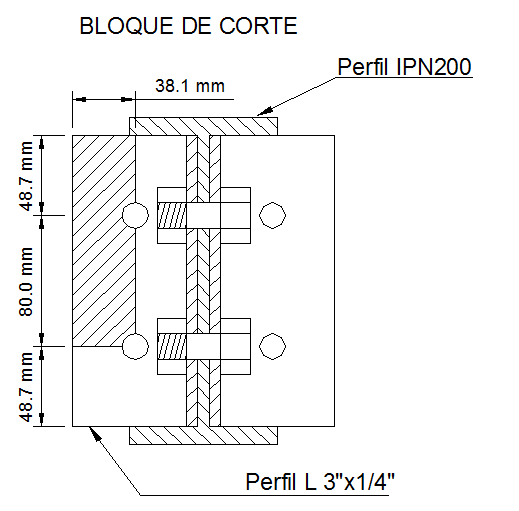
\includegraphics[scale = 0.6]{chapters/chapter_1/images/Bloque_de_Corte_3.png}
\end{center}
\caption{Bloque de Corte}
\end{figure}

\end{itemize}
\end{enumerate}